\chapter{引言}
\label{chap:introduction}

\section{什么是机器学习}
\label{sec:what-is-machine-learning}

\subsection{什么是学习}

孩子见过几只猫和狗后，可能认出另一只没有见过的猫；学生练习解方程，希望把解题方法
用于新的方程；驾驶员根据路况和操作反馈调整驾驶行为。三个例子有一个共同点：过去的经历
改变了以后处理问题的方式。我们用“学习”描述这些现象时，关注的是经验留下了什么可以
保持的能力，而不只是当时答对了多少次；疲劳或兴奋也会改变一次操作的结果，但这种短暂
波动不足以说明发生了学习。

这些例子引出本章要回答的核心问题：只经历过一部分情形，为什么可能更好地处理尚未经历的情形？

哲学研究经验与知识的关系时，已经提出过这个问题。\term{演绎}（deduction）要求结论由给定前提
保证；\term{归纳}（induction）则从已经观察到的情形形成更广的判断。D.~Hume（休谟）讨论过
归纳的困难：过去发生的事情，不能仅凭演绎就保证在未来继续发生\scite{hume1748}。任何从有限
经验推出新判断的做法，都要跨过这一步；而要跨过它，除了经验本身，还需要某些假设，规定
哪些关系可以延续到没有观察过的情形。后文会看到，机器学习程序同样离不开这样的假设。

哲学关心经验能否支持结论；要判断学习是否真的发生，还需要选定可以观察的变化。心理学可以
考察行为是否改变，也可以研究经验怎样改变知识和表征，即组织与理解信息的方式。
\term{条件作用}（conditioning）研究刺激、反应和结果之间形成的联系，例如得到奖励的行为
以后可能更频繁地出现；认知取向还关注记忆、概念和策略的变化。De~Houwer等人提出的功能性
定义，以环境规律引起的行为改变来界定学习\scite{dehouwer2013}。这些研究表明，学习包含的
变化比记住事实更广，也可以借助可观察的行为改变来界定。

\subsection{从学习到机器学习}
邮件的写法持续变化，靠人工逐条补充关键词和例外，很难维护一套充分的拦截规则。与此同时，
过去收到的邮件及其处理结果已经留下了记录。我们希望程序利用这些记录调整判断规则，再用新
邮件检验调整的效果。\term{机器学习}（machine learning, ML）研究的正是这类利用经验改变程序
行为的问题。它沿用学习的基本直觉，但不要求程序复制人的心理过程；可利用的经验也不限于
已有记录，还可以来自与环境交互得到的反馈。

把学习交给程序，就要说明两件事：程序怎样从有限的已知记录得到处理新情形的规则，以及用什么证据
判断规则是否有效。从已见邮件推测新邮件的类别，正是前面所说的归纳跨越。
图~\ref{fig:learning-process-scene}概括了这一过程。已经核实类别的历史邮件（训练样本）
按一套事先写定的调整办法（学习规则）确定判断规则，得到训练模型；训练模型固定后，代入新邮件
的信息得到预测；另留的一批已知类别的邮件（评价样本）再检查预测是否符合真实类别。训练时
答对与评价时答对来自不同的邮件，是两项不同的证据：规则本来就是照着训练邮件调出来的，
在这些邮件上分类正确，并不等于它能正确处理没有参与训练的邮件。
第~\ref{sec:spam-classification-example}节将沿这个例子逐一给出这些名称的准确含义。

\begin{figure}[htbp]
  \centering
  
\includegraphics[width=\linewidth]{figures/03-foundations/01-basics/generated/learning-process-scene/figure.png}
  \caption{从历史经验到新邮件预测的学习过程。左侧核实历史邮件标签，中间按学习规则形成训练模型，
  右侧对新邮件预测并用独立评价样本检验结果。邮件图标、人物和分类场景均为示意，
  不表示某个图标能够确定真实类别，也不表示评价标签参与本次训练。}
  \label{fig:learning-process-scene}
\end{figure}

早期研究从不同对象出发探索这种可能性。McCulloch和Pitts研究理想化神经元构成的网络，
Turing讨论通过教育和经验培养机器，Rosenblatt的感知机根据分类错误调整连接权重，
Samuel的跳棋程序利用棋局记录和自我对弈改进决策
\scite{mcculloch1943,turing1950,rosenblatt1958,samuel1959}。后两项工作分别依据分类对错和
对弈胜负调整程序，是按已知答案学习和通过交互学习的早期例子。

这些探索表明程序能够随经验改变，但还留下三个问题：这种改变在新样本上有什么保证，参数
怎样实际求出，以及选择时能够利用输入中的哪些信息。此后的研究分别回应了它们。Vapnik和
Chervonenkis等人把有限样本提供的统计保证与候选规则的复杂度联系起来，研究在怎样的抽样
条件与候选复杂度下，训练所得规则对新样本有保证\scite{vapnik1971}。训练多层网络面临求解
参数的计算问题，\term{误差反向传播}（error backpropagation）沿计算关系反向求出学习目标
函数对参数的梯度，为参数更新提供所需导数\scite{rumelhart1986}。输入怎样表示同样影响学习
结果：\term{表示学习}（representation learning）让模型从数据中学习输入到内部特征的转换，
\term{深度学习}（deep learning）用多层参数化变换学习这类表示及其上的任务规则，在数据、
计算和模型规模扩大后得到广泛应用\scite{lecun2015}。

说明一个学习系统，需要同时借助不同学科的工具。\term{人工智能}（artificial intelligence）研究智能任务与行动；\term{概率论}（probability theory）和\term{统计学}（statistics）帮助描述不确定性并从有限记录估计规律；\term{优化}（optimization）研究怎样求解参数选择问题。信息论、信号处理和控制分别提供编码与表示、信号变换和反馈分析工具，数据系统承担采集、存储与计算。\term{数据挖掘}（data mining）也使用分类、聚类和\term{异常检测}（anomaly detection），侧重在已有数据中发现可用模式。应用领域则规定答案的含义、错误代价和使用限制。

这些联系说明，仅给出模型名称还不足以描述一个机器学习问题；我们还要交代系统完成什么任务、利用什么经验、按什么标准评价。下面的定义把这三项固定下来。

\subsection{机器学习的定义}

判断经验是否带来了改进，需要把比较说清楚。同一个程序可以执行多项任务，同一次调整
也可能降低一种错误而增加另一种错误。因此，我们要同时规定任务、衡量结果的标准和
程序所用的经验。T.~M.~Mitchell的经典定义把这三项合在一起\scite{mitchell1997}。

\begin{definition}[机器学习]
\label{def:machine-learning}
对于某类任务 $T$ 和性能度量 $P$，如果一个计算机程序在任务 $T$ 上按 $P$ 衡量的性能
因经验 $E$ 而有所改善，就称该程序从经验 $E$ 中进行了学习。
\end{definition}

定义~\ref{def:machine-learning}中的三个要素各有具体含义：

\begin{itemize}
  \item \term{任务}（task, $T$）说明希望系统完成什么，例如判断邮件是否为垃圾邮件；
  \item \term{性能度量}（performance measure, $P$）说明怎样判断任务完成得好不好，
    例如分类正确的比例或漏放垃圾邮件的数量；
  \item \term{经验}（experience, $E$）说明系统从什么信息中学习，例如带人工标签的
    历史邮件，也可以是没有标签的数据、用户反馈或与环境交互得到的奖励。
\end{itemize}

三项要素对应判断“学没学到”时必须回答的三个问题：比的是哪件事，用什么尺子比，改变来自
哪些信息。缺了任何一项，“程序变好了”都无法核对。改变其中一项，学习问题也可能随之改变。
同一批历史邮件既能用于判断垃圾邮件，也能用于整理主题，这是任务不同；一个分类器准确率较高，
被错判为垃圾邮件的正常邮件却仍可能超出可接受范围，这说明换一种性能度量，结论也会不同。

定义中的“改善”，是利用指定经验前后按$P$作出的比较判断：同一程序在接触$E$之前有一个成绩，
接触之后有另一个成绩，后者更好才算学习。下一节的邮件分类器就是这样比较的：不读任何历史
邮件、总是回答“正常邮件”的程序，在一组测试邮件上分对$62.5\%$；用历史邮件调整规则后，
同一组邮件上分对$75\%$。$E$可以是一整批样本、交互记录或其他反馈，不限于逐个加入的样本；
增加一次经验仍可能使某次评价下降，定义并不要求性能随经验数量逐步、单调地提高。

\section{例子：垃圾邮件分类}
\label{sec:spam-classification-example}

现在把任务、经验和性能度量落实到同一个分类过程：用已标注的历史邮件选择判断规则，再让
选定的规则处理未参与选择的邮件，依次观察数据准备、建模、训练、预测和评估各自改变了什么。
这里的邮件及标签都是教学构造，后面报告的是这套构造数据上的计算结果，不能据此估计真实
邮件系统的分类效果。

这个系统读取一封邮件中的可用信息，并在垃圾邮件和正常邮件之间作出判断。两个候选类别构成\term{二分类}（binary classification）问题。历史邮件的已知类别用\term{标签}（label）记录：垃圾邮件记为$1$，称为\term{正类}（positive class）；正常邮件记为$0$，称为\term{负类}（negative class）。正负名称只是计算约定，不表示哪一类更好或更重要。表~\ref{tab:spam-three-elements}据此列出本例的任务、性能度量和经验，供后面的训练与评价共同使用。

\begin{table}[htbp]
  \centering
  \small
  \begin{tabularx}{\linewidth}{@{}lX@{}}
    \toprule
    \textbf{要素} & \textbf{在垃圾邮件分类中的含义} \\
    \midrule
    任务 $T$ & 输入一封邮件，输出“垃圾邮件”或“正常邮件”。 \\
    性能度量 $P$ & 考察测试邮件中分类正确的比例，并分别记录误拦正常邮件和漏放垃圾邮件。 \\
    经验 $E$ & 历史邮件、由人工给出的类别标签，以及据此形成的训练反馈。 \\
    \bottomrule
  \end{tabularx}
  \caption{垃圾邮件分类问题的任务、性能度量与经验。三个要素共同规定了“学得更好”的含义。}
  \label{tab:spam-three-elements}
\end{table}

为了判断训练是否带来收益，我们先指定一个可以直接执行的比较方案，称为\term{基线}
（baseline）。本例的基线始终预测训练样本中数量较多的正常邮件。
若测试样本也以正常邮件为主，它可以靠这一固定答案取得较高准确率，却漏掉全部垃圾邮件。
因此，比较时除了准确率，还要分别数出误拦和漏放，才能判断学到的规则解决了什么问题。

\subsection{从邮件到样本与特征}

一封原始邮件不能直接用作分类模型的输入，我们需要先决定程序能够读取哪些信息。
把邮件转换成模型可处理的对象，就得到它的\term{表示}（representation）；用来描述邮件
的各个量称为\term{特征}（feature）。例如，可以记录发件人和域名、主题与正文中的词语、
字符组合、链接、附件、邮件头、发送时间及历史通信关系。现实系统会综合多种信息，
某一项线索是否可靠仍取决于使用环境，不能只看特征的名称就断定它有效。

为使预测计算可以手工核对，我们只保留两个计数：正文中的促销提示词次数$x_1$与外部链接数
$x_2$。模型实际读取的量称为\term{预测输入}，本例中一封邮件的预测输入于是成为$\bm{x}=(x_1,x_2)^{\top}\in\mathbb{R}^{2}$。
这两项只提供部分线索。教学数据允许相同或相近计数对应不同标签，真实邮件的类别也不能
由这两个数唯一决定。简化表示舍去了发件人身份、语境和附件内容，后面的模型都受到
这项信息限制。

把一封邮件的预测输入与已知标签放在一起，就得到一条带标签的记录$z_i=(\bm{x}_i,y_i)$，也称样本点，其中$i$表示邮件编号，标签是可供对照的答案。一批记录按采集顺序组成\term{样本}$D=(z_1,\ldots,z_n)$，顺序和重复记录都保留；\term{数据集}（dataset）是保存这批记录的常用工程名称。表~\ref{tab:spam-data-excerpt}同时列出原始片段和预测输入计数，便于检查二者的区别：
片段属于收集到的信息，计数向量则是按当前表示规则从中提取的预测输入。

\begin{table}[t]
  \centering
  \footnotesize
  \begin{tabularx}{\linewidth}{@{}llXcccl@{}}
    \toprule
    \textbf{编号} & \textbf{用途} & \textbf{邮件片段} & $x_1$ & $x_2$ & $y$ & \textbf{类别} \\
    \midrule
    \code{tr01} & 训练 & “限时优惠，立即领取……” & 3 & 2 & 1 & 垃圾邮件 \\
    \code{tr06} & 训练 & “周会改至下午三点” & 0 & 0 & 0 & 正常邮件 \\
    \code{tr11} & 训练 & “优惠券报销说明” & 2 & 0 & 0 & 正常邮件 \\
    \code{va02} & 验证 & “会员权益，详情见链接” & 1 & 2 & 1 & 垃圾邮件 \\
    \code{va03} & 验证 & “本周三场促销培训” & 3 & 0 & 0 & 正常邮件 \\
    \code{te02} & 测试 & “两项优惠，见附件链接” & 2 & 1 & 0 & 正常邮件 \\
    \code{te07} & 测试 & “专属优惠今日有效” & 2 & 0 & 1 & 垃圾邮件 \\
    \code{te08} & 测试 & “优惠详情见两个链接” & 1 & 2 & 0 & 正常邮件 \\
    \bottomrule
  \end{tabularx}
  \caption{教学记录的部分节选。$x_1$为促销提示词次数，$x_2$为外部链接数，
  标签 $y=1$ 表示垃圾邮件。训练样本、验证样本和测试样本承担不同职责。}
  \label{tab:spam-data-excerpt}
\end{table}

表中还有一列“用途”，它回答的是：同一批带标签记录能否既用来选规则，又用来报告规则的好坏？
设想一位学生拿到考卷后先背熟答案再作答，高分只说明他记住了这张卷子，说明不了他会解新题。
程序也一样：参数是照着某批邮件调出来的，再用这批邮件打分，选择时针对它们得到的好处会被
算进成绩，使评价偏乐观。所以至少要把“用来选择”的记录和“用来检验”的记录分开。

只分两组还不够，因为选择发生在两个层次。第一层是在给定设置下调整参数；第二层是挑选设置
本身，例如训练多少步。若用检验组挑选设置，检验组又参与了选择。因此，我们在训练开始前把
邮件分成三组：\term{训练样本}（training sample）用于学习参数，\term{验证样本}（validation
sample）用于在几种设置之间作比较和挑选，\term{测试样本}（test sample）留到所有选择完成后
作一次独立评价。验证样本和测试样本合称\term{评价样本}，二者用途不同，需要分开保留。
同样的分工也约束预处理：若需要估计词表或特征尺度，只能在训练样本上拟合。词频筛选和均值
计算都属于利用数据作出选择；把测试信息用于这些步骤，就已经破坏了预留评价的分工。

\subsection{对问题进行建模}

两个计数还不能给出类别，我们需要约定怎样把它们合成判断依据。本例先计算线性得分：\term{偏置}（bias）$b$给出两个计数都为零时的得分，\term{权重}（weight）$w_1,w_2$分别说明促销词或链接增加一个时得分改变多少。偏置与权重的具体取值要由训练确定，这类需要根据数据确定的数称为\term{模型参数}（model parameter）。

得分可取任意实数，本身没有概率含义。前面的样本已经表明，相同计数可能对应不同标签：
表~\ref{tab:spam-data-excerpt}中\code{te08}与\code{va02}的计数都是$(1,2)$，类别却相反。
既然两个计数不能唯一确定类别，更合理的做法是承认这种不确定，让模型回答“计数为$(x_1,x_2)$
的邮件中，垃圾邮件大约占多大比例”，即估计给定计数时标签为1的可能性。

要把“可能性”写成数学对象，需要用随机变量描述一封随机到来的邮件。记它的特征向量为$\bm{X}$，
取值在$\mathbb{R}^2$中；它的标签为$Y$，取值在$\{0,1\}$中。大写字母表示尚未观察到的随机量，
小写的$\bm{x}$表示某封具体邮件已经算出的特征值。把模型参数记为
$\bm{\theta}=(b,w_1,w_2)^{\top}\in\Theta$，本例取$\Theta=\mathbb{R}^3$。只取$0$或$1$的随机
变量由“取$1$的概率”一个数就能完全描述，这种分布称为Bernoulli分布。于是可以约定
$Y\mid\bm{X}=\bm{x}\sim\operatorname{Bernoulli}(p_{\bm{\theta}}(\bm{x}))$：给定邮件特征后，
标签为$1$的概率是$p_{\bm{\theta}}(\bm{x})$，标签为$0$的概率是$1-p_{\bm{\theta}}(\bm{x})$。

剩下的问题是怎样由得分算出这个概率：得分落在整条实数轴上，概率却必须落在$0$与$1$之间。
本例用\term{逻辑函数}（logistic function）完成这一转换：得分越大，输出越接近1；得分越小，
输出越接近0；得分为$0$时输出恰为$0.5$。这个计算关系写为
\begin{align}
  s_i &= b+w_1x_{i,1}+w_2x_{i,2}, \\
  p_{\bm{\theta}}(\bm{x}_i)
  =f_{\bm{\theta}}(\bm{x}_i)
  =\hat{p}_i
  &=\sigma(s_i)=\frac{1}{1+\exp(-s_i)}.
  \label{eq:spam-model}
\end{align}
式中的$\exp(-s_i)=e^{-s_i}$是指数函数，$\sigma$是逻辑函数的简写。这样的分类\term{模型}（model）
规定了预测输入与预测输出之间的计算关系。$\hat{p}_i$之所以能解释为模型对“第$i$封邮件是
垃圾邮件”的概率估计，依据的是上述Bernoulli条件假设；仅仅把任意得分压到$(0,1)$内，
并不自动获得概率含义。

概率还需要转换成类别：当$\hat{p}_i\geq 0.5$时预测$\hat{y}_i=1$，否则预测$\hat{y}_i=0$。
这里预先选取$0.5$作为分类\term{阈值}（threshold），决定多大的概率估计被归为垃圾邮件；邮件服务再依据应用策略决定是否拦截。
这个取值便于演示，但不表示在误拦与漏放成本不对称时仍然最优。

阈值规则还可以换回得分来看。逻辑函数随得分严格递增，且$\sigma(0)=0.5$，所以
$\hat{p}_i\geq 0.5$当且仅当$s_i\geq 0$。在$(x_1,x_2)$平面上，方程$b+w_1x_1+w_2x_2=0$是一条
直线，直线一侧的邮件判为垃圾邮件，另一侧判为正常邮件。这条分开两类预测的线称为
决策边界（decision boundary）。改变参数就是移动或转动这条直线，训练要做的正是
确定它的位置。

三个模型参数合在一起就是$\bm{\theta}$；一组$\bm{\theta}\in\Theta$对应一个具体函数，把所有允许参数对应的函数合在一起，就得到\term{候选模型类}（candidate model class），预测问题中也称为假设空间（hypothesis space）$\mathcal{H}=\{f_{\bm{\theta}}:\bm{\theta}\in\Theta\}$。它是训练可以从中挑选的全部规则：例如$\bm{\theta}=(-1,1,0)^{\top}$对应“只看促销词，至少有一个就判为垃圾邮件”的规则，$\bm{\theta}=(-1,0,1)^{\top}$则只看链接是否至少有一个，两者都是$\mathcal{H}$的成员。因此，写出式~\eqref{eq:spam-model}只确定了候选范围；训练还要在这个范围内选择具体参数。

为什么要预先划定候选范围，而不让数据自己决定一切？因为样本并不能直接给出新邮件的答案。
多种规则可以在已见样本上作出相同判断，却在未见的预测输入上分歧。例如，训练记录中没有
计数为$(3,3)$的邮件；一条规则把它判为垃圾邮件，另一条在其余位置都相同、只在$(3,3)$处
判为正常邮件，两条规则对全部历史记录给出的结论完全一样，单凭记录无法在二者之间取舍。
只查看计数的规则与还查看发件人的规则，也可能同样符合历史记录。

要作出取舍，就必须在数据之外先作一些规定。本例预先选择了两个计数、线性得分、逻辑函数
和固定阈值：线性得分意味着决策边界只能是直线，上面那种只在一个点上翻转结论的规则根本
不在候选之中。这些使某些规律优先于另一些规律的选择称为\term{归纳偏置}（inductive bias），
可以理解为学习者在看到数据之前就带有的“倾向”。即使在限定的逻辑模型中求得唯一参数，这种
唯一性也来自模型形式、学习目标和选择规则共同施加的限制。第~\ref{sec:what-is-machine-learning}节
所说的归纳跨越，在算法中就体现为归纳偏置：它规定算法怎样超出有限记录作出判断，也规定
算法不能利用什么。本例对计数相同的邮件总给出相同预测；如果真正的区别在发件人或语境中，
再怎样调整权重，也不能恢复表示时已经舍去的信息。

本例的学习目标是让模型给真实邮件类别分配较高概率。候选规则给出不同概率，要选择参数，就需要把这一目标转成可计算的评价。\term{损失函数}（loss function）
给一次预测的错误程度计分，损失越小，表示这次预测越符合目标。本例输出的是概率，
这里采用\term{二分类交叉熵}（binary cross-entropy）：它检查模型给真实类别分配了多少
概率，分配得越少，惩罚越大。对于标签$y_i\in\{0,1\}$，损失写为
\begin{equation}
  \ell(\hat{p}_i,y_i)
  =-y_i\log\hat{p}_i-(1-y_i)\log(1-\hat{p}_i).
  \label{eq:binary-cross-entropy}
\end{equation}
这里$\log$取自然对数。以一封真正的垃圾邮件为例，它的标签为$y_i=1$，损失为$-\log\hat{p}_i$。
如果模型预测它是垃圾邮件的概率为 $0.9$，损失约为 $0.105$；如果预测概率只有 $0.1$，
损失则约为 $2.303$。这两个数值把惩罚方向具体显示出来：真实类别得到的概率越小，交叉熵损失越大。
对正常邮件$y_i=0$，第一项消失，损失变为$-\log(1-\hat{p}_i)$，惩罚的是模型给“垃圾邮件”
分配了过多概率。式中的两项因此只有一项起作用，$y_i$充当开关。

为什么用对数而不直接用$1-\hat{p}_i$之类的差值？在Bernoulli假设下，模型给真实标签$y_i$分配的
概率可以统一写成$\hat{p}_i^{\,y_i}(1-\hat{p}_i)^{1-y_i}$，交叉熵正是这个概率取对数后的相反数。
若各封邮件的标签相互独立，整批标签的联合概率是各封概率的乘积，取对数后乘积变为求和。
所以，使下面的平均交叉熵最小，等价于使模型给整批训练标签分配的联合概率最大，也就是统计中
最大似然估计的做法。

参数要服务于整批训练邮件，不能只凭一封邮件的损失选择。对于训练样本中的$n$条记录，对损失取平均，得到\term{经验风险}（empirical risk），用它概括模型在整批训练邮件上的错误代价。“风险”沿用统计决策理论的说法，指平均损失；“经验”表示这个平均只在已经观察到的记录上计算：
\begin{equation}
  \hat{R}_{\mathrm{train}}(\bm{\theta})
  =\frac{1}{n}\sum_{i=1}^{n}\ell\bigl(f_{\bm{\theta}}(\bm{x}_i),y_i\bigr).
  \label{eq:spam-empirical-risk}
\end{equation}
以$\Theta$为候选范围，以经验风险为学习目标函数，按其值从小到大选择参数，称为\term{经验风险最小化}
（empirical risk minimization, ERM）。如果最小值能够取到，这个目标可以写为
\begin{equation}
  \hat{\bm{\theta}}
  \in\argmin_{\bm{\theta}\in\Theta}\hat{R}_{\mathrm{train}}(\bm{\theta}).
  \label{eq:spam-erm}
\end{equation}
这里的$\argmin$表示使目标函数达到最小值的参数集合；有限计算下的训练通常只能寻找近似解，而不一定得到这个集合中的参数。学习目标规定参数选择的方向，性能度量用于任务评价，二者可以相同，
也可以不同。本例用交叉熵训练模型，评价整个任务时却要看测试样本上的准确率、误拦数和漏放数。

\subsection{根据历史邮件进行训练}

经验风险给出比较标准，程序还需要具体的参数更新规则。\term{训练}（training）指利用训练样本选择参数，并按规定的停止条件和取出最终参数的方式形成训练模型。本例采用\term{梯度下降}（gradient descent）：计算当前学习目标函数的梯度，沿其反方向移动，再在新位置重复计算。从
$\bm{\theta}^{(0)}=(0,0,0)^{\top}$开始，更新规则为
\begin{equation}
  \bm{\theta}^{(t+1)}
  =\bm{\theta}^{(t)}-\eta\nabla_{\bm{\theta}}
  \hat{R}_{\mathrm{train}}\bigl(\bm{\theta}^{(t)}\bigr).
  \label{eq:spam-gradient-update}
\end{equation}
上标$(t)$表示第$t$次更新后的参数；$\nabla_{\bm{\theta}}$表示对参数求梯度，即由目标函数对
$b,w_1,w_2$的三个偏导数组成的向量。\term{学习率}（learning rate）$\eta$控制每一步的幅度，
本例取$\eta=0.35$。

为什么沿梯度的反方向走能降低目标值？记$\bm{g}$为当前梯度。由多元函数的一阶泰勒展开，
参数移动一个小量$\bm{\delta}$后，目标值约改变$\bm{g}^{\top}\bm{\delta}$。取$\bm{\delta}=-\eta\bm{g}$，
改变量约为$-\eta\lVert\bm{g}\rVert^2$，只要梯度非零就为负。本例的学习目标函数具有连续的导数，
这一近似在步长足够小时可靠，所以沿非零梯度的反方向走足够小的一步会使目标值下降；步子过大时，
被忽略的高阶项可能占上风，目标值未必下降。

对本例的模型，梯度有简单的形式。由$\sigma'(s)=\sigma(s)\bigl(1-\sigma(s)\bigr)$可以算出，单封邮件
的交叉熵对得分的导数恰为$\hat{p}_i-y_i$；再由$s_i$对$b,w_1,w_2$的偏导数分别为$1,x_{i,1},x_{i,2}$，得到
\begin{equation}
  \nabla_{\bm{\theta}}\hat{R}_{\mathrm{train}}(\bm{\theta})
  =\frac{1}{n}\sum_{i=1}^{n}(\hat{p}_i-y_i)
  \begin{pmatrix}1\\x_{i,1}\\x_{i,2}\end{pmatrix}.
  \label{eq:spam-gradient}
\end{equation}
预测概率比真实标签高，$\hat{p}_i-y_i>0$，更新就把这封邮件的得分往下压；反之往上抬。每封邮件
推动参数的力度与它的预测误差成正比，并按它的计数分配到各个权重上。

更新公式说明了参数怎样一步步变化，却没有回答每步走多远、一共走多少步。权重和偏置由式~\eqref{eq:spam-gradient-update}学习，学习率与更新次数则要另外设定。这类控制模型或学习过程、需要人为选定的配置称为\term{超参数}（hyperparameter）。阈值也可以通过验证选择；本例把它预先固定为$0.5$，它只参与类别判断，不参与交叉熵更新。

本例只用验证样本选择更新次数：在$C=\{20,40,60\}$三个迭代时点中，以验证准确率较高者为优，平局时采用更新次数较少者。这样，模型选择的候选范围、评价量和选择规则都在训练前确定下来，算法~\ref{alg:spam-training}把它们与参数更新写在一起。

\begin{algorithm}[垃圾邮件分类器的训练]
  \label{alg:spam-training}
  \begin{algorithmic}[1]
    \Require 训练样本 $D_{\mathrm{train}}$，验证样本 $D_{\mathrm{val}}$，
      学习率 $\eta$，候选迭代次数集合 $C=\{20,40,60\}$，分类阈值 $0.5$
    \Ensure 选定参数 $\hat{\bm{\theta}}$
    \State 初始化 $\bm{\theta}^{(0)}$
    \For{$t=0,\ldots,\max(C)-1$}
      \State 在训练样本上计算经验风险及其梯度
      \State 按式~\eqref{eq:spam-gradient-update}得到 $\bm{\theta}^{(t+1)}$
      \If{$t+1\in C$}
        \State 保存候选参数 $\bm{\theta}^{(t+1)}$，并按阈值 $0.5$ 记录验证准确率
      \EndIf
    \EndFor
    \State 从验证准确率最高的候选中选取迭代次数最小者，记为 $\hat t$
    \State 令 $\hat{\bm{\theta}}=\bm{\theta}^{(\hat t)}$
    \State \Return $\hat{\bm{\theta}}$
  \end{algorithmic}
\end{algorithm}

第一步可以手工复核。初始参数全为零，所有邮件的得分都是$0$，$\hat{p}_i=0.5$，每封邮件的交叉熵都是$\log 2\approx0.693$。12封训练邮件中有5封垃圾邮件，代入式~\eqref{eq:spam-gradient}，偏置分量为$(12\times0.5-5)/12=1/12$；5封垃圾邮件的$x_1$之和为11、全部12封的$x_1$之和为15，故$w_1$分量为$(0.5\times15-11)/12\approx-0.292$；同理$w_2$分量为$(0.5\times18-11)/12\approx-0.167$。乘以$-\eta=-0.35$，参数约为$(-0.029,0.102,0.058)^{\top}$，学习目标值降为$0.658$。两个权重变为正数，说明促销词和链接越多，模型越倾向判为垃圾邮件。

这一步降低了目标值，却不能决定何时停止。我们在第20、40和60次更新时分别保存参数；三份参数是同一模型形式在不同训练阶段的版本，验证邮件只用于比较这些版本，始终不参与梯度计算。用三个版本分别分类6封验证邮件：第20和40次更新各分类正确5封，准确率为$5/6$；第60次只分类正确4封，准确率为$4/6$。最高准确率在前两个时点并列，平局规则选中第20次更新，供后续预测使用的参数为
\begin{equation}
  \hat{\bm{\theta}}=(-1.000,\,0.692,\,0.230)^{\top}.
  \label{eq:spam-fitted-parameters}
\end{equation}
完整的12封训练邮件、6封验证邮件和8封测试邮件及更新计算保存在随书图源程序\texttt{introduction-spam-example.py}中，位置为\url{figures/03-foundations/01-basics/tikz/introduction-spam-example.py}。该程序按这里的初始化、学习率和检查点复算参数与曲线；正文表格只节选记录，显示值由完整计算结果舍入。

\begin{table}[htbp]
  \centering
  \small
  \begin{tabularx}{\linewidth}{@{}rXXXX@{}}
    \toprule
    $t$ & $b^{(t)}$ & $w_1^{(t)}$ & $w_2^{(t)}$ & 学习目标值 \\
    \midrule
    0  & $0.000$  & $0.000$ & $0.000$ & $0.693$ \\
    1  & $-0.029$ & $0.102$ & $0.058$ & $0.658$ \\
    20 & $-1.000$ & $0.692$ & $0.230$ & $0.452$ \\
    \bottomrule
  \end{tabularx}
  \caption{训练过程中参数与学习目标值的变化；这里的目标函数为平均交叉熵。第20次迭代是验证样本选定的检查点；
  表中数值由完整计算结果舍入得到。}
  \label{tab:spam-training-record}
\end{table}

继续训练时，图~\ref{fig:spam-training-loss}中的训练交叉熵仍在下降，验证交叉熵也逐渐降低。但第60次更新的验证准确率反而低于第20次更新。概率改变可以降低交叉熵，也可能使某封邮件的概率越过$0.5$阈值，从分对变成分错。这个计算例子说明，训练目标与类别评价关注的量不同，学习目标值下降不能直接替代准确率检查。

\begin{figure}[htbp]
  \centering
  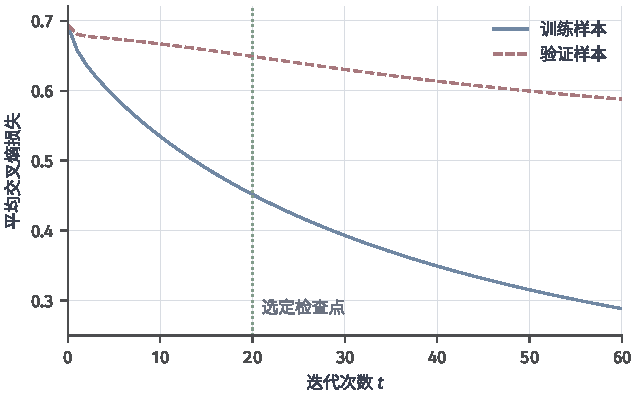
\includegraphics[width=\linewidth]{figures/03-foundations/01-basics/matplotlib/introduction-training-loss/figure.pdf}
  \caption{训练样本和验证样本上的平均交叉熵损失。蓝色实线表示训练曲线，红色虚线表示验证曲线，
  绿色竖线标出按验证准确率选定的第20次迭代；模型选择并非直接读取学习目标值的最低点。}
  \label{fig:spam-training-loss}
\end{figure}

这次计算涉及三样容易混在一起的东西：参数未定的形式、得到参数的办法，以及得到的结果。式~\eqref{eq:spam-model}属于第一样，它规定候选模型的预测输入与预测输出关系，但参数尚未确定。\term{学习规则}（learning rule）规定怎样从数据得到参数：候选范围、训练目标、初始化、参数更新、停止条件和最终参数的取出方式，本例的停止位置由验证样本选定。学习规则的可执行实现称为\term{学习算法}（learning algorithm），算法~\ref{alg:spam-training}就是本例的具体程序。将选定参数填入候选形式，才得到\term{训练模型}，即训练后实际使用的预测函数。训练模型固定以后，它可以反复处理新邮件，无须在每次预测时重新选择参数。

\subsection{对新邮件进行预测}

现在固定训练模型，读取一封没有参与训练的邮件。把邮件的预测输入代入训练模型，得到\term{预测输出}，这一过程称为\term{预测}（prediction）。本例先计算垃圾邮件概率，再按阈值给出预测类别；过程不读取真实标签，也不更新参数。未标注的新邮件和已标注的测试邮件都可以这样计算，只有取得真实标签后才能评价预测是否正确。是否据此放行、隔离或删除邮件，则是使用预测结果的行动决策，需要另外规定错误代价和权限。

我们先计算\code{new01}，它有两个促销词和两个链接，预测输入为$\bm{x}=(2,2)^{\top}$。使用已选参数，得到
\begin{align}
  s&=-1.000+0.692\times 2+0.230\times 2=0.844,\\
  \hat{p}&=\sigma(0.844)=0.699.
\end{align}
计算所得概率越过$0.5$阈值，所以预测类别为垃圾邮件。表~\ref{tab:spam-inference-results}
列出三个新样本的结果。

\begin{table}[htbp]
  \centering
  \small
  \begin{tabularx}{\linewidth}{@{}lXcccl@{}}
    \toprule
    \textbf{编号} & \textbf{邮件片段} & $(x_1,x_2)$ & $\hat{p}$ & \textbf{阈值} & \textbf{预测类别} \\
    \midrule
    \code{new01} & “会员优惠，点击两个链接” & $(2,2)$ & $0.699$ & $0.5$ & 垃圾 \\
    \code{new02} & “项目文档见共享链接” & $(0,1)$ & $0.316$ & $0.5$ & 正常 \\
    \code{new03} & “优惠详情见两个链接” & $(1,2)$ & $0.538$ & $0.5$ & 垃圾 \\
    \bottomrule
  \end{tabularx}
  \caption{新邮件的预测结果。概率和类别均由式~\eqref{eq:spam-fitted-parameters}
  中的固定参数计算；真实标签不属于预测所需的信息。}
  \label{tab:spam-inference-results}
\end{table}

如果要在另一处重现同样的预测，仅保存参数向量并不够。训练与预测还必须沿用相同的特征定义和预处理顺序。如果训练时$x_1$来自固定词表，换一份词表后同一邮件的输入可能改变，原参数便不再对应原计算。部署时应一并保存参数、表示规则和阈值，才能保持预测的含义。

\subsection{模型的评估}

预测新邮件时，我们并不知道它们的真实类别，只看输出无法判断预测是否正确。我们因此使用此前预留的带标签测试邮件，在参数与阈值固定后逐封预测，再与真实标签对照。表~\ref{tab:spam-test-results}列出全部8封邮件。测试标签只服务于这次评价；若根据结果回头调整参数或配置，这组邮件就参与了选择，失去原先独立检验的作用。

\begin{table}[htbp]
  \centering
  \footnotesize
  \begin{tabularx}{\linewidth}{@{}lcccc>{\raggedleft\arraybackslash}X@{}}
    \toprule
    \textbf{编号} & $(x_1,x_2)$ & $y$ & $\hat{p}$ & $\hat{y}$ & \textbf{结果} \\
    \midrule
    \code{te01} & $(3,2)$ & 1 & $0.823$ & 1 & 识别垃圾邮件 \\
    \code{te02} & $(2,1)$ & 0 & $0.649$ & 1 & 误拦正常邮件 \\
    \code{te03} & $(1,3)$ & 1 & $0.594$ & 1 & 识别垃圾邮件 \\
    \code{te04} & $(0,0)$ & 0 & $0.269$ & 0 & 放行正常邮件 \\
    \code{te05} & $(0,2)$ & 0 & $0.368$ & 0 & 放行正常邮件 \\
    \code{te06} & $(1,0)$ & 0 & $0.424$ & 0 & 放行正常邮件 \\
    \code{te07} & $(2,0)$ & 1 & $0.595$ & 1 & 识别垃圾邮件 \\
    \code{te08} & $(1,2)$ & 0 & $0.538$ & 1 & 误拦正常邮件 \\
    \bottomrule
  \end{tabularx}
  \caption{独立测试样本上的逐样本预测。测试标签只用于比较，不参与参数、迭代次数或阈值的选择。}
  \label{tab:spam-test-results}
\end{table}

逐行计数得到6次正确分类，准确率为$6/8=75\%$。3封垃圾邮件全部被识别，同时有2封正常邮件被误拦。相同测试样本上，始终预测正常的基线分类正确5封，准确率为$62.5\%$；它没有误拦，却漏放了3封垃圾邮件。与基线相比，学到的模型提高了这里的准确率、减少了漏放，但也增加了误拦。应用是否接受这一取舍，要由两类错误的实际代价决定。

\begin{table}[htbp]
  \centering
  \small
  \begin{tabularx}{\linewidth}{@{}Xccc@{}}
    \toprule
    \textbf{方法} & \textbf{准确率} & \textbf{误拦数} & \textbf{漏放数} \\
    \midrule
    学到的线性模型 & $75.0\%$ & 2 & 0 \\
    全部预测为正常 & $62.5\%$ & 0 & 3 \\
    \bottomrule
  \end{tabularx}
  \caption{学到的模型与基线在同一测试样本上的比较。单个指标不能完整表达两类错误的代价。}
  \label{tab:spam-baseline-comparison}
\end{table}

把同一组参数放到训练邮件上，12封中分对11封（只有\code{tr11}被误判），准确率约$91.7\%$；
测试邮件上的准确率则是$75\%$。两个数字的差别提醒我们，训练成绩回答的是“照着答案调过的题
做得怎样”，测试成绩回答的才是“没见过的题做得怎样”。模型把从有限样本学到的规律用到同一
来源的新样本上的能力，称为\term{泛化}（generalization）；测试评价的就是它。

训练成绩好而新样本上差，是需要警惕的一种情形。设想一个“查表”分类器：它逐条记住每封训练
邮件的计数和标签，遇到记过的计数就照抄，没见过的一律判为正常。只要训练记录的标签互不冲突，
它在训练邮件上全部答对，对新邮件却几乎没有判断力。模型追随了训练样本的偶然细节，在训练
样本上错误很少，在同一来源的新样本上错误却明显增多，这种情形称为\term{过拟合}（overfitting）。
本例中也能看到类似的苗头：继续训练到第60次更新，训练邮件全部分对，验证邮件却只分对4封。
不过验证邮件只有6封，单凭这一点差别不足以作出确定判断。

相反的情形是训练与新样本上的结果都差，模型可能没有学到数据中的主要规律，称为
\term{欠拟合}（underfitting）。直观地说，候选规则越多而训练记录越少，越容易碰巧找到一套
贴合偶然细节的规则，出现过拟合；候选范围太窄时，主要规律可能根本不在候选之内，训练不足时
则可能还没有被找到，两者都会造成欠拟合。两种情形需要对照训练与验证上的结果分别诊断：
只看一次较差的测试成绩，既不能判断属于哪种情形，也不能分辨欠拟合来自表达能力受限还是训练不足。

限制模型追随偶然细节的一种方式是\term{正则化}（regularization）：在选择参数时加入约束，例如惩罚绝对值过大的权重。在当前线性得分中，权重的绝对值越大，一个计数的微小变化对得分的影响越大。一种常见写法是把学习目标改为$\hat{R}_{\mathrm{train}}(\bm{\theta})+\lambda(w_1^2+w_2^2)$，其中$\lambda\geq0$控制惩罚强度，本身是需要用验证样本选择的超参数；$\lambda=0$时退回原来的经验风险最小化。惩罚权重幅度，便是在进一步降低原学习目标值与限制这种敏感性之间取舍。这种惩罚只是在既定表示之内调整参数的取舍，表示阶段舍去的发件人、语境等信息仍然无法找回，也不能据此认定权重越小泛化就越好。收益是否符合当前任务，仍应通过验证样本判断。

测试样本只代表当前来源的邮件，未来的邮件未必服从同样的规律。发送者更换措辞、用户群体改变，或部署渠道不同，都可能改变输入与标签出现的规律，这种改变称为\term{分布变化}（distribution shift）。即使模型没有过拟合，旧测试样本也可能不能代表新的使用环境。要发现这种失效，只看无标签输入和模型输出并不可靠：输入和人群监测能提供线索，延迟取得的标签或抽样复核才能直接检查预测错误。是否需要补充数据、改变表示或重新训练，要靠这样的持续评价来判断。

回顾整个案例：表示决定模型能看到什么，模型形式与学习目标决定候选范围和选择方向，训练与验证选出参数，独立测试再把收益和错误分开呈现。换成其他应用时，这些环节仍然存在，但输入、所需结果和错误代价会改变。下面三节依次回到任务、经验与性能度量，说明邮件案例中哪些选择可以推广，哪些必须随问题重新确定。

\section{任务}
\label{sec:machine-learning-tasks}

一批用户评论可以用于判断满意度、提取产品名称，也可以用于生成摘要；同样的材料并不规定唯一的工作。因此，描述任务时要说明系统读取什么、产生什么结果，以及结果在什么情境中使用。怎样评价这些结果仍由性能度量$P$规定，任务$T$不代替评价标准。不同应用要求的输出各不相同，但其中反复出现的几种输出形式可以提炼出来跨应用复用；我们先看应用，再做提炼。

\subsection{应用场景中的任务}

\paragraph{自然语言处理}
客服收到一句“我的订单什么时候到”，可能需要判断查询意图、找出订单信息或组织答复。输入都是语言，所需输出却不同。\term{自然语言处理}（natural language processing, NLP）用计算方法分析和生成人类语言；以下文本例子说明输出要求如何决定任务。

如果答案是预先规定的一类，就可以采用\term{文本分类}（text classification）。例如，\term{情感分析}（sentiment analysis）把“送货很快，包装也完好”判为正面评价，\term{垃圾信息检测}（spam detection）判断消息是否属于垃圾内容，\term{意图识别}（intent recognition）把订单到达时间的询问归为物流查询。若手中只有反馈文本，还没有给定类别答案，可以按内容关系分组，再观察各组对应的主题。这称为\term{文本聚类}（text clustering）。分类依据已规定的类别作答，聚类则探索尚未确定的分组。

一句话的整体类别有时不足以完成处理。系统还可能需要说明每个词或片段的作用，因而采用\term{序列标注}（sequence labeling），为文本各位置赋标签。\term{词性标注}（part-of-speech tagging）判断名词、动词等词类；\term{命名实体识别}（named entity recognition）定位人名、机构名、地名等片段并给出类型，也常借助这种任务形式。

标出了片段，还可以进一步建立可供后续使用的事实记录。\term{信息抽取}（information extraction）从文本中取得实体、关系等结构化信息。在“小林就职于星海公司”中识别人名与机构后，\term{关系抽取}（relation extraction）判断二者的任职关系，可将实体对作为输入进行关系分类。序列标注与信息抽取的多个输出互有联系，因此属于\term{结构化预测}（structured prediction）：预测结果是一个有内部关系的整体，而非互不关联的单个答案。

文字不同也可能表达同一需求。“如何退货”和“商品不想要了怎么退”能否使用同一答复，需要比较含义。\term{语义匹配}（semantic matching）判断文本是否意思相近，或查询是否与文档相关。若只输出匹配与否，任务是分类；若估计连续的相似程度，可以作为\term{回归}（regression）；若据此排列候选文档，则属于\term{排序}（ranking），关注相对次序。\term{自然语言推断}（natural language inference）考察陈述间的关系，常用蕴含（entailment）、矛盾（contradiction）和中性（neutral）表示前文支持后文、彼此冲突或信息不足。例如，按通常语境，“一名运动员正在跑步”支持“有人正在运动”。这里的判断依赖语言背景，不能直接等同于形式逻辑的演绎。

输出也可以是一段新文字。\term{文本生成}（text generation）根据输入要求组织文本；\term{机器翻译}（machine translation）在保留含义的前提下转换语言，\term{文本摘要}（text summarization）从长文中形成短概述，\term{智能问答}（question answering）根据问题和资料形成答案。用输入限定生成结果时，称为\term{条件生成}（conditional generation）。这些应用并不只有生成这一种表述：\term{抽取式摘要}（extractive summarization）选择原文句子，可以采用分类或排序；选取材料中的答案片段，则可以采用信息抽取。\term{生成式摘要}（abstractive summarization）和\term{生成式问答}（generative question answering）才要求模型自行组织输出文字。

\paragraph{图像处理}
照片也可以支持不同的输出要求。相册管理要判断照片属于海滩还是街道，道路感知还要定位行人和道路。\term{图像处理}（image processing）以图像或视频帧为对象，其中的学习任务既可以识别内容，也可以生成和恢复图像。

要给整幅图像赋类别，可以采用\term{图像分类}（image classification）。相册按海滩、街道或室内场景分类，质检系统判断表面是否有缺陷，都是这类任务。输出可以是一个类别，也可以包含多个类别；这种要求通常不包括对象的具体坐标。

道路上是否有行人与行人在何处，是两个不同问题。\term{目标检测}（object detection）同时预测对象类别和位置，常用包围对象的矩形，即\term{边界框}（bounding box），定位汽车、行人或交通标志。类别由分类预测，框的位置和大小常由回归预测。图中对象数目也可能变化，所以完整输出是一组检测结果，需要同时确定数量与对应关系。

若要知道道路或器官的精确轮廓，矩形框又过于粗略。\term{图像分割}（image segmentation）把输出细化到像素区域。\term{语义分割}（semantic segmentation）为每个像素赋予道路、建筑或天空等类别标签，可视为有关联的像素分类；\term{实例分割}（instance segmentation）进一步分开同类对象，例如为每位行人保留各自轮廓。医学影像勾画器官时，也需要这种比大致位置更精细的区域信息。

分析动作还要说明身体各部位的排列。\term{姿态估计}（pose estimation）预测关键位置或空间姿态；人体的肩、肘、膝等明确位置称为\term{关键点}（keypoint）。这些位置用于描述动作并支持运动分析和人机交互。可以直接回归坐标，也可以先预测关键点在各位置出现的可能性，再确定位置。各点之间受到身体结构关系约束，因而整个结果同样属于结构化预测。

以图像为输出时，还要区分产生新内容与恢复已有观测。按文字绘制插图属于\term{图像生成}（image generation）；根据受损或不完整观测去噪、补全区域、提高分辨率，则属于\term{图像重建}（image reconstruction）。重建可以回归像素，也可以在观测约束下进行条件生成。观测丢失了信息时，可能存在多个符合约束的结果，生成的细节未必就是原场景中的细节。

\paragraph{推荐、搜索与广告}
电影应用可以在用户尚未输入片名时，依据观看记录、评分和当前情境，主动给出待观看列表。这样的过程称为\term{推荐}（recommendation）：从大量物品中选择可能对用户有用的对象并呈现。“物品”可以是电影、商品或新闻。这里的困难是需求尚未被完整表达，系统需要从行为与情境推测当前兴趣，再决定展示什么。

用户也可能直接输入“适合孩子看的太空电影”。\term{搜索}（search）以这样的查询为线索，从内容集合中查找满足信息需求的对象。查询既可以是词语或句子，也可以是图片。搜索电影时，系统读取查询与电影资料，输出相关电影列表，属于\term{信息检索}（information retrieval）\scite{manning2008ir}。它需要在有限时间内理解查询条件、取得候选，并让较相关的结果排在前面。

若页面还允许广告主付费推广，选择对象时就多了新的参与方和限制条件。\term{广告}（advertising）从有投放资格的广告中分配展示机会，除了判断用户可能作出的响应，还要处理广告主的受众条件、出价和预算，以及平台审核、计费和用户体验规则。系统需要先判断资格，再估计点击或购买等价值，最后在资源与规则约束下决定展示和收费，并检验产生的效果。

推荐、搜索和广告都从大量对象中选择，因而可以共享用户信息、内容特征与交互记录，并复用理解需求、取得候选、预估价值、排序和利用反馈等环节。不过，三者对同一对象的判断可能不同。喜欢科幻片的用户可能愿意看太空惊悚片，但它未必满足“适合孩子”的查询；与兴趣相符的广告，还要经过审核并满足定向和预算条件。推荐主要推测潜在需求，搜索受当前查询约束，广告还受到付费关系与资格规则约束，共享计算环节并不使这些目标等价。要说明机器学习在其中具体预测什么，需要把目标分解到可计算的环节。下面沿需求理解、候选筛选和结果展示的依赖顺序考察，每一步都交代输入、输出与用途。

搜索首先需要从查询中取得对象和条件，称为\term{查询理解}（query understanding）。对“适合孩子看的太空电影”，文本分类可以识别找电影的意图，信息抽取或序列标注可以取出太空题材和孩子这一受众条件。输入是查询文本，输出的类别或片段为检索提供依据。推荐则从历史行为与当前情境估计兴趣；广告还要解析受众条件和内容。它们共同为后续匹配形成需求侧与对象侧的表示。

有了需求表示，仍不宜对全部内容作精细计算。\term{候选生成}（candidate generation），也称\term{候选召回}（candidate retrieval），先选出一小批可能有用的对象，以限制后续计算。推荐匹配用户与物品，搜索匹配查询与物品；广告还要先执行审核、定向和预算筛选。模型可以利用交互或相关性标签学习匹配得分，例如比较用户兴趣与电影资料、查询与电影简介，或用户情境与广告信息。得分用来筛选集合，留下有用且合格的对象，再交给后续环节。

留下候选后，可以进一步估计用户的评价与行为。\term{评分预测}（rating prediction）读取用户和物品信息，估计评分数值，通常可用回归表述。\term{点击率预测}（click-through rate prediction）估计展示后发生点击的概率，历史点击与未点击记录可以作为二分类标签。\term{转化率预测}（conversion rate prediction）估计在约定条件下购买等行为的概率，例如点击商品后购买的概率。三类应用都可能使用这些量，但点击概率只回答点击问题，不能直接代表查询相关性、用户满意度或广告的增量效果。

候选的分数最终要形成一份有次序的列表。\term{学习排序}（learning to rank）根据相关性标签、偏好或交互反馈学习次序，例如让儿童科幻片排在太空惊悚片之前，以满足当前查询。模型读取需求与候选信息，产生得分或相对次序，评价则关注有用结果的位置。推荐比较当前用户的物品价值，搜索比较查询相关性，广告还须结合出价、预算和展示限制。竞价与分配同时处理展示资格和计费，超出了预测分数排序。最终列表还可以经过\term{重排序}（reranking）或混合编排，减少重复、兼顾多样性或限制广告密度；这些调整既可使用模型，也可依据明确规则\scite{googleRecommendationOverview}。

历史行为的时间顺序也可能影响当前选择。\term{序列推荐}（sequential recommendation）根据按时间排列的记录预测用户下一次会感兴趣的内容：连续浏览儿童动画后，用户当前需求可能偏离长期偏爱的科幻题材。只预测下一项时，可以使用分类或排序；若还要评价当前展示对后续观看和长期体验的影响，就要比较多次行动的后果，形成\term{序贯决策}（sequential decision making）。广告预算消耗和重复曝光同样会影响后续机会，当前收益便需要与未来机会一起考虑。

这些环节的输出可以成为下一环节的输入：需求与对象表示支持匹配，候选集合缩小比较范围，行为预测支持排序，排序、竞价或编排决定展示，反馈再支持调整。学习模型并非每一步的必要条件，关键词检索和广告资格规则仍可直接执行。利用反馈时还要检查交互标签是怎样产生的：前排结果更容易被看到和点击，点击量同时受到位置与既有展示策略影响，不能直接解释为相关性、偏好或广告效果\scite{joachims2016biased}。

\paragraph{其他领域}
上述输入虽有差别，分类、数值预测和行动选择却可以反复出现。科学研究与工业系统也会提出相近任务，只是观测形式与使用约束不同。下面用生命科学、自动化与控制、语音处理说明这种跨领域复用。

生命科学（life sciences）可以从细胞测量、基因表达（gene expression）和分子结构形成输入。\term{细胞类型识别}（cell type identification）按测量特征判断类别，属于分类；按基因表达模式组织细胞，则可采用聚类。\term{分子性质预测}（molecular property prediction）估计溶解度等数值性质，可采用回归；\term{分子生成}（molecular generation）根据所需性质提出结构，属于生成。模型的预测与候选结构仍需要领域知识和实验验证，计算输出本身并不构成科学结论。

自动化与控制系统（automation and control systems）也可以把观测转为明确任务。\term{故障诊断}（fault diagnosis）依据传感器记录判断故障类别；\term{系统辨识}（system identification）从记录学习动态关系，例如由当前温度与加热功率预测后续温度，其中的数值输出可用回归。机器人控制则随环境与自身状态连续选择动作，属于序贯决策，常把感知、状态预测与行动选择合在一起。

\term{语音处理}（speech processing）改变的是输入输出材料。\term{语音识别}（speech recognition）把连续音频转换成文字序列，涉及\term{序列预测}（sequence prediction）；\term{语音合成}（speech synthesis）按文本产生音频，属于条件生成。

这些领域的例子说明，\term{应用场景}（application scenario）是问题的使用环境，任务则是系统在其中必须完成的具体工作。同一场景可以包含数项任务，同一任务形式也可以服务多个场景；下一小节就把反复出现的任务形式单独整理出来。

\subsection{常见任务类型}

前面的应用反复用到几种基本输出：类别、数值、分组和低维表示，分别对应\term{分类}（classification）、回归、聚类和降维四类任务。排序、生成、结构化预测和序贯决策的输出或目标更复杂，可以在局部调用这四类任务，但仍要单独规定完整结果的要求。表~\ref{tab:common-ml-tasks}列出这种基础与复合关系；这里的“基础”说明可分解的计算职责，并不表示复合任务等同于某一种基础任务。

以文本生成为例说明复合任务怎样调用基础任务。文本首先被切成\term{词元}（token），即分词规则得到的文本处理单位，可以是字、词或子词。生成时可以把输入和已经生成的片段作为条件，在词元表中预测下一个词元，再将选中的词元接到片段末尾，如此逐个词元地产生整段文字。这意味着生成一段文字在局部上反复调用分类（从词元表中选一个词元）；但整段文字是否连贯、是否符合要求，并不能由逐个词元的准确率完整评价，仍需按复合任务自身的标准衡量。

\begin{table*}[t]
  \centering
  \small
  \begin{tabularx}{\linewidth}{@{}llXXX@{}}
    \toprule
    \textbf{层次} & \textbf{任务} & \textbf{典型输出} & \textbf{任务要求} & \textbf{例子} \\
    \midrule
    基础 & 分类 & 一个或多个离散类别 & 判断输入属于哪些类别 & 垃圾邮件识别、图像分类 \\
    基础 & 回归 & 连续数值 & 使预测值接近目标数值 & 评分预测、需求预测 \\
    基础 & 聚类 & 样本的组别或结构 & 按相似性探索分组结构 & 文档主题探索、用户分群 \\
    基础 & 降维 & 低维表示 & 用较少变量保留主要结构 & 数据可视化、压缩 \\
    复合 & 排序 & 相关性分数或候选次序 & 把更有用的对象排在前面 & 文档检索、推荐排序 \\
    复合 & 生成 & 文本、图像、音频等对象 & 产生符合条件或规律的内容 & 摘要、翻译、图像生成 \\
    复合 & 结构化预测 & 相互关联的标签或数值 & 联合满足输出内部关系 & 序列标注、目标检测 \\
    复合 & 序贯决策 & 随状态变化的一系列行动 & 提高一段时间内的累计回报 & 机器人控制、交互式推荐 \\
    \bottomrule
  \end{tabularx}
  \caption{四类基础任务与常见复合任务。复合任务可以调用基础任务，但其整体输出与评价目标不能由局部任务替代。}
  \label{tab:common-ml-tasks}
\end{table*}

分类先由任务规定类别集合及其含义，再判断输入属于哪一类或哪些类。邮件二分类在垃圾与正常之间选择；\term{多分类}（multiclass classification）可以在正面、负面、中性等互斥类别中选择；\term{多标签分类}（multilabel classification）则允许一张照片同时带有海滩、日落和人物标签。模型需要从输入找出区分类别的依据，类别名称本身并不提供判断规则。

实际分类器常先计算分数或概率，再用最大分数、阈值等规则给出类别。连续的中间分数仍服务于离散决策，并不会把最终任务改成回归。各类别所占比例、不同错误的代价，以及一个输入能否同时携带多个标签，会影响决策和评价方式。若逐词或逐像素分类，输出位置之间还可能有关联，完整任务就需要处理这些关系。

回归把输出改为连续数值，例如价格、用电量、观看时长或未来温度。模型可读取一条记录或一段历史，预测一个数或一组有关联的数。数值相差多少通常比落入哪个类别更重要；因此，还要根据量纲与使用代价，决定用绝对差、平方差还是相对差评价误差。

单个温度预测值只给出了点预测，还没有说明温度可能波动多大。需要不确定性时，必须另加分布或预测区间及对应评价。分类中的连续得分则只用于支持类别决策，不能只看模型输出了数值，就把任务当成回归。也可以把连续目标切成区间后分类，但区间内差异随之被舍去，原来比较误差大小的标准也发生了变化。

没有预先给出的类别答案时，可以从样本关系探索分组，称为\term{聚类}（clustering）。输入是一批样本及其表示，输出可以是组别，也可以是层次结构。形成分组前，要先规定怎样比较样本：文档可用词语或语义表示，用户可用行为或属性。表示、相似性或分组目标改变，同一批记录的分组也可能改变。

分组还需要决定数量与归属方式。组数可以预先设定，也可以由数据与停止规则共同决定；每个样本可以只归入一组，也可以对多个组保留归属程度。由于没有预定的唯一组别答案，评价应检查组内集中、组间分离、对数据变化的稳定性或后续分析用途，不能直接套用分类准确率。分类与聚类虽都能输出组别，区别在于组别体系是任务给定的，还是从样本关系探索得到的。

若困难来自输入变量太多，可以用\term{降维}（dimensionality reduction）把$\bm{x}\in\mathbb{R}^{d}$变为$\bm{u}\in\mathbb{R}^{k}$，其中$k<d$。较少变量有利于显示、存储和后续计算，也可能舍弃部分信息；是否有损取决于映射和数据结构，例如冗余坐标可以在降维后由其余坐标恢复。要选择降维结果，必须说明保留目标：重建输入、保持距离或邻域，以及保留区分类别所需信息，提出的是不同要求。

这些要求未必同时满足。适合二维显示的表示可能难以精确重建，保留总体变化最大方向也可能舍去少数类别的线索。降维产生的新表示可以交给分类、回归或聚类，而聚类本身产生分组。两者能够组合；改变表示可能改变距离和分组，也可能在只去除冗余变量时保持当前数据的关系，所以应按照实际后续用途检查信息保留与损失。

排序最终比较候选次序，分数的绝对大小未必是评价目标。学习排序有三种组织方式。\term{逐点方法}（pointwise approach）分别预测每个候选的相关类别或程度，再据分数排列；\term{成对方法}（pairwise approach）比较两个候选谁应在前，可将这一关系作为二分类；\term{列表方法}（listwise approach）则按整个列表的结果组织学习。这些转化使分类与回归工具可用于排序，但结果仍应按候选位置评价。

\term{生成}（generation）需要产生文本、图像或音频等整体对象。前面的文本生成例子已经说明，自回归生成（autoregressive generation）把已生成的词元接回条件中，再预测并续接下一个词元，直到满足停止条件；连续信号生成可调用回归，并利用降维或聚类得到的表示。完整评价仍关注对象是否符合条件和数据规律。结构化预测也组合局部任务，例如目标检测结合类别与位置预测，序列标注还要处理相邻标签关系。序贯决策则将范围扩展到多次行动：分类可选择动作，回归可估计回报，聚类或降维可概括状态，但最终要比较一段时间内的累计收益。

基础任务提供可以组合的计算部件，并不替代应用目标：推荐可以先估计点击概率，检测可以同时分类与回归，低维表示可以继续用于分组。每次分解都要检查局部输出是否保留原问题需要的信息，并按完整任务评价最终结果。

\subsection{任务与学习范式}
\label{sec:task-and-learning-paradigm}

任务规定输入与输出，却没有规定怎样学会完成它。即使任务固定为文本分类，我们可以直接使用带标签文本训练分类器，也可以先从无标签文本学习表示，再用少量标签训练分类器；两种方式得到相同类型的答案，使用的经验和反馈却不同。\term{学习范式}（learning paradigm）描述经验与训练的组织方式，与规定输入输出的任务分别承担职责。

区分范式，可以沿三个问题追问：学习所对照的答案从哪里来，反馈是否来自行动，经验以什么方式到达。

第一个问题看答案从哪里来。配对答案可以来自人工标注，也可以来自成交记录或随后观测到的天气，并不以人工给出为必要条件。邮件案例中，已知类别直接告诉模型每个输入应当输出什么，这属于\term{监督学习}（supervised learning）。若只有无标签文本，没有任何答案可对照，只能探索记录之间的结构，则采用\term{无监督学习}（unsupervised learning）。介于两者之间的是从记录自身造出答案：遮住文本的一部分，用保留下来的原文作为答案来预测被遮住的内容，就得到了可比较的目标，这属于\term{自监督学习}（self-supervised learning）。在同一任务中结合少量标签和大量无标签记录，则可采用\term{半监督学习}（semi-supervised learning）。

第二个问题看反馈是否来自行动。下棋或控制机器人时，系统要先行动，再观察后果，通常没有人逐步告诉它哪一步才正确。依据后果与奖励调整决策属于\term{强化学习}（reinforcement learning）；若能观看专家怎样做，主要依据动作示范学习，则属于\term{模仿学习}（imitation learning）。

第三个问题看经验怎样到达。邮件案例一次拿到全部记录；若经验陆续到达，每次更新还要保留仍然需要的旧能力，这由\term{持续学习}（continual learning）研究。

这些名称分别着眼于反馈来源、可用任务标签的多少及其取得方式，以及经验到达的方式，划分维度不同，因而可以组合，不能仅凭“文本”或“推荐”等应用名称判断。描述一个系统时，应把使用环境、所需结果和学习方式分别说清：一个场景可以包含多种任务，一项任务也可以利用不同形式的经验学习。第~\ref{chap:machine-learning-paradigms}章将用这些区分建立范式之间的比较依据。

\section{经验}
\label{sec:machine-learning-data}

邮件分类器读取的只是两个计数，但学习过程还用到了标签、样本划分和预处理规则，而且每条信息只允许用于特定环节。样本、反馈与交互中可供学习使用的部分构成经验，数据是它们在系统中的载体。本节先说明记录的来源、分布与质量，确定经验覆盖什么情形；再说明对象怎样被记录并转换为预测输入，确定程序能利用什么信息；最后说明数据在哪个阶段可见，检查选择与评价能否分开。

\subsection{数据来源、分布与质量}
\label{sec:experience-data-distribution}

要用有限的邮件记录评价未来表现，需要先规定记录与未来邮件遵循什么共同规律。\term{数据分布}（data distribution）给输入和标签的各种组合赋概率，描述哪些情形更常出现；数据集只是按某种采样方式留下的有限记录。二者之间的关系取决于采样条件，不能仅凭记录数量多，就认定数据集代表了分布。

常用分析把这一关系简化为\term{独立同分布}（independent and identically distributed, i.i.d.）：样本中的各条记录相互独立，并服从同一记录分布。可以把它想象成从同一个装满邮件的箱子里有放回地反复抽取：每次抽取不受前几次影响（独立），箱子的内容始终不变（同分布）。这两项条件之所以重要，是因为它们让有限记录上的平均值成为总体平均的可靠估计：由概率论中的大数定律，只要单条记录的期望损失有限，对固定模型而言，独立同分布记录上的平均损失随记录数增加而趋近总体的平均损失，第~\ref{sec:performance-measures}节的期望风险正是这个总体平均。这两项条件支持许多经典统计工具，但实际数据常常不满足：相邻传感器读数可能相关，不同用户可能服从不同规律，邮件写法也可能随时间改变。面对这些情况，需要明确依赖、群组或变化，再选择相应工具；独立同分布不成立并不等于数据不能分析。

即使无法精确写出分布，也能检查记录是否覆盖目标场景。来自同一狭窄渠道的大量样本，仍可能缺少某类用户、设备或环境。测量误差与标注分歧影响可靠性，类别不平衡则会让少量重要事件在总体计数中被掩盖。补充数据时，应据目标范围查找缺失情形，并检查测量和标签；仅重复已有来源未必补上这些缺口。

\subsection{数据表示与使用}
\label{sec:experience-data-representation}

邮件案例中，一封实际邮件是原始对象，保存的正文、发件人、时间和附件字段是记录；计数规则把记录转换为预测输入$\bm{x}_i$，与标签$y_i$组成带标签的记录$(\bm{x}_i,y_i)$。经验也可以由无标签对象、偏好对、行动轨迹或奖励组成，不必都化为输入与单个标签的配对。

用$o$记待处理对象，表示规则$r$将它转换为$x=r(o)\in X$，其中$X$是预测输入的取值空间。表示决定算法可以利用哪些差异：词数和链接数没有保留词序与语境，像素没有直接标出对象边界，类别编号的大小通常也不代表对象间的差别。后续模型仅凭转换后的输入，无法找回已经舍去的信息。

文本还可以通过编码器转换为向量，这类向量表示常称为\term{嵌入}（embedding）。检索系统可以比较查询与文档向量的相似程度，分类器也可以将向量作为输入。向量应保留哪些信息、几何上的接近能否表示含义相近，都需要由训练目标、数据与实际用途支持。

\subsection{数据划分与使用边界}
\label{sec:experience-data-boundary}

表示决定模型读取什么，数据划分则规定这些信息在什么阶段可见。邮件案例保留的三组记录各有分工：训练样本用于学习参数和拟合词表、归一化系数等预处理规则，验证样本用于选择超参数、比较候选模型和决定何时停止，测试样本只在所有选择完成后估计最终系统对未见数据的表现。

除了分成几组，还要决定按什么方式分，这取决于希望把结论推广到哪些对象。图~\ref{fig:data-split-uses}按时间组织数据，适用于预测后续邮件的设定。随机划分常用于近似同分布数据；若要评价未来时段，或推广到未见用户，就应按时间或用户划分，避免让未来信息或同一用户记录同时影响训练和测试。

\begin{figure*}[htbp]
  \centering
  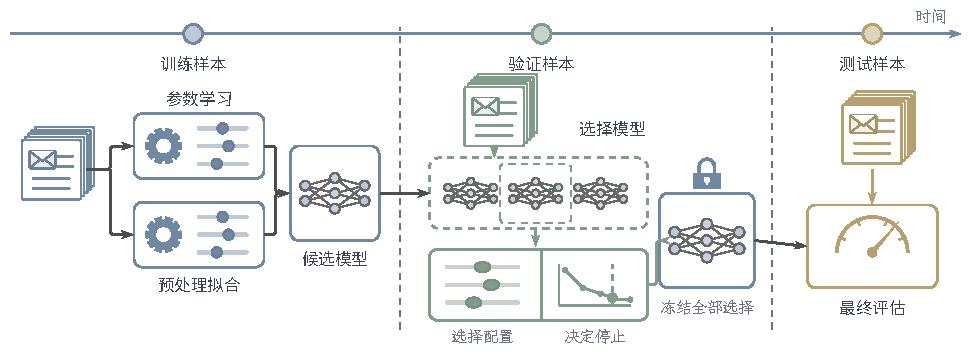
\includegraphics[width=164.600mm]{figures/03-foundations/01-basics/tikz/introduction-data-split/figure.pdf}
  \caption{训练样本、验证样本和测试样本的用途。时间箭头表示一种面向未来预测的划分方式；记录数量仅作示意，不代表划分比例。训练样本用于参数学习与预处理拟合，验证样本用于配置和停止位置的选择，测试样本在这些选择冻结后才用于最终评估。}
  \label{fig:data-split-uses}
\end{figure*}

一旦选择过程使用了原本预留的信息，就发生\term{信息泄漏}（information leakage）。邮件副本跨入训练与测试两组，可能让模型靠记忆答对；用全体记录拟合词表，也把测试信息用于了输入选择。反复看测试结果再改模型，同样使最终选择依赖这组测试记录，它便不能继续充当独立证据。三种情形的共同点是：选择过程使用了本应保留给评价的信息，可能使报告成绩产生乐观偏差。偏差并不保证每次都出现或必定为正，但此时原有的独立评价解释已经失效，不能再把这组成绩当作未参与选择的新邮件表现。

避免泄漏只恢复了选择与评价的分工，还没有保证测试分布代表所有未来环境。用户、设备或时间范围改变后，仍应重新验证并监测。解释成绩时，要把数据来源、生成过程与使用条件同记录本身一起报告。

\section{性能度量}
\label{sec:performance-measures}

误拦重要邮件与漏放垃圾邮件可能造成不同代价，而第~\ref{sec:spam-classification-example}节的准确率只汇总正确比例，掩盖了两类错误的构成，不足以决定是否采用系统。要把应用要求转为数量，先确定哪些结果需要分别比较，再选择指标与基线。

把真实类别与预测类别交叉计数，就能区分这两类错误。这张表称为\term{混淆矩阵}（confusion matrix），四格分别记录两种正确判断和两种错误。垃圾邮件为正类时，真正例（true positive, TP）是正确拦截，假正例（false positive, FP）是误拦正常邮件，假负例（false negative, FN）是漏放垃圾邮件，真负例（true negative, TN）是正确放行。表~\ref{tab:spam-confusion-matrix}由此前表~\ref{tab:spam-test-results}逐行计数，因而可以直接复核。

\begin{table}[htbp]
  \centering
  \small
  \begin{tabular}{@{}llcc@{}}
    \toprule
    & & \multicolumn{2}{c}{\textbf{预测类别}} \\
    \cmidrule(l){3-4}
    & & 垃圾邮件 & 正常邮件 \\
    \midrule
    \textbf{真实类别} & 垃圾邮件 & TP $=3$ & FN $=0$ \\
                    & 正常邮件 & FP $=2$ & TN $=3$ \\
    \bottomrule
  \end{tabular}
  \caption{垃圾邮件测试结果的混淆矩阵。行表示真实类别，列表示预测类别；
  “垃圾邮件”被约定为正类。}
  \label{tab:spam-confusion-matrix}
\end{table}

这四格支持三种不同的比例：全体邮件中分类正确的比例、被拦邮件中确属垃圾的比例，以及垃圾邮件中被识别的比例。三者分别称为\term{准确率}（accuracy）、
\term{精确率}（precision）和\term{召回率}（recall）。\term{$F_1$值}（F1 score）用
精确率和召回率的调和平均数综合二者，较小的一项会限制这个综合值。例如精确率为$1$、召回率只有$0.02$时，算术平均约为$0.51$，像是“还过得去”；调和平均却约为$0.04$，如实反映出几乎没有识别垃圾邮件。按上述分母取比例，计算为
\begin{align}
  \text{准确率}
    &=\frac{\mathrm{TP}+\mathrm{TN}}
      {\mathrm{TP}+\mathrm{FP}+\mathrm{FN}+\mathrm{TN}},\\
  \text{精确率}
    &=\frac{\mathrm{TP}}{\mathrm{TP}+\mathrm{FP}},\\
  \text{召回率}
    &=\frac{\mathrm{TP}}{\mathrm{TP}+\mathrm{FN}},\\
  F_1
    &=\frac{2\mathrm{TP}}{2\mathrm{TP}+\mathrm{FP}+\mathrm{FN}}.
  \label{eq:classification-measures}
\end{align}
在本例中，准确率为 $6/8=0.75$，精确率为 $3/5=0.60$，召回率为 $3/3=1.00$，
$F_1=0.75$。召回率为1说明测试样本里的垃圾邮件都被识别出来；精确率只有0.60说明被拦截的
5封邮件中有2封其实是正常邮件。

当精确率和召回率都有定义且二者之和非零时，$F_1$的计数式等于二者的调和平均数。使用这些
公式时还需检查分母：如果没有邮件被预测为正类，精确率就不能直接按此计算；如果测试样本中
没有正类，召回率也同样如此。采用计数式时，只要$2\mathrm{TP}+\mathrm{FP}+\mathrm{FN}>0$，本书就以该式定义$F_1$；因此$\mathrm{TP}=0$且$\mathrm{FP}+\mathrm{FN}>0$时取值为0。三项全为0时分母为零，本书将$F_1$报告为“不适用”而不任意置零。使用软件工具时也应说明其退化情形约定。

准确率怎样掩盖少数类别，可以用一个构造例子说明：一万封邮件中若只有十封垃圾邮件，全部放行也有$99.9\%$准确率，却没有识别任何垃圾邮件。精确率与召回率改用不同分母，分别暴露误拦与漏放，但$F_1$仍没有直接计入实际代价。

两类错误还可以通过阈值相互交换。保持模型的概率输出不变而提高阈值，拦截集合只会缩小或不变，召回率不会增加；精确率是否增加，取决于新被排除的邮件中垃圾与正常邮件的比例。仅为说明这一点，可以在表~\ref{tab:spam-test-results}上把阈值改为$0.6$（这不是一次阈值选择）：概率为$0.594$与$0.595$的两封垃圾邮件和概率为$0.538$的一封正常邮件不再被拦截，被拦的只剩\code{te01}和\code{te02}。召回率由$1$降为$1/3$，精确率也由$0.60$降为$0.50$。提高阈值本想减少误拦，这里误拦只少了一封，却多漏放了两封垃圾邮件。因此，阈值应在验证样本上依据代价选择，测试样本只检验选定结果。

对数值预测，评价可以从预测与真实值的偏差建立。\term{平均绝对误差}
（mean absolute error, MAE）对偏差的绝对值取平均，\term{均方误差}
（mean squared error, MSE）则对偏差的平方取平均。对评价样本中的$n$条记录，记真实值为$y_i$、
预测值为$\hat{y}_i$，则
\begin{align}
  \operatorname{MAE}
    &=\frac{1}{n}\sum_{i=1}^{n}|\hat{y}_i-y_i|,\\
  \operatorname{MSE}
    &=\frac{1}{n}\sum_{i=1}^{n}(\hat{y}_i-y_i)^2.
\end{align}
平方相对于绝对值更强调较大的偏差，两个指标因此给出不同的误差权重。排序、生成和序贯决策也各有相应指标，评价时还可能需要结合人工判断、延迟、资源消耗和长期影响。本章不逐一罗列，只强调指标必须与任务和使用条件相匹配。

无论哪种指标，都来自有限的测试记录，应用关心的却是目标环境里的预测。至此我们已经见过单次损失及其样本平均：式~\eqref{eq:binary-cross-entropy}给出一次预测的损失，式~\eqref{eq:spam-empirical-risk}把它在训练样本上取平均，得到经验风险。要描述模型在未来邮件上的表现，需要按未来输入和标签的概率规律取平均，得到\term{期望风险}（expected risk，也称population risk），即模型在目标分布上的平均损失。前面用测试成绩讨论的泛化，关心的正是这个总体量。记随机输入及其标签为$(\bm{X},Y)$，目标分布为$\mathcal{P}$，则
\begin{equation}
  R(\bm{\theta})
  =\mathbb{E}_{(\bm{X},Y)\sim\mathcal{P}}
  \left[\ell\bigl(f_{\bm{\theta}}(\bm{X}),Y\bigr)\right].
  \label{eq:expected-risk}
\end{equation}
式中的$\mathbb{E}$表示取期望，也就是按各种情形出现的概率对损失加权平均。目标分布一般无法直接获得，独立测试记录因而用来估计这一平均量或对应的任务指标。这里“独立”是关键：若测试记录从$\mathcal{P}$独立抽取，且训练模型的选择没有用到它们，那么模型已经固定，测试平均损失的期望恰为$R(\bm{\theta})$，没有偏向。训练平均则不同，$\hat{\bm{\theta}}$本来就是照着训练记录选出的，$\hat{R}_{\mathrm{train}}(\hat{\bm{\theta}})$通常低估$R(\hat{\bm{\theta}})$；二者差多少、何时可以控制，是理论部分要研究的问题。测试估计也只适用于相应的采样条件，不能保证任意未来环境中的表现。

由此也得到比较模型时的几条要求：使用相同的数据划分、可用信息和评价口径；预处理方案与阈值可用验证样本选择，词表、均值等参数仍只用训练样本拟合；报告时交代选择方式与估计的不确定性。

\section{本章小结}
\label{sec:introduction-summary}

本章开头问：只经历过一部分情形，为什么可能更好地处理尚未经历的情形？邮件案例给出的回答是，有限经验本身不足以决定对新情形的判断，还要几项选择共同作用：表示决定保留什么信息，模型形式与归纳偏置规定候选关系，学习规则利用训练样本形成训练模型。检验时，再固定参数与配置，用没有参与选择的记录计算任务指标。这个过程既得到了可执行的分类规则，也暴露了误拦代价；它给出了检验泛化的方法，但无论训练成绩还是测试成绩，都不能单独证明规则对所有未来邮件有效。

任务、经验和性能度量共同规定学习问题。任务说明系统要产生什么结果，经验说明可用的信息及其使用边界，性能度量说明怎样比较结果；数据与未来使用环境的关系，则决定测试成绩能外推到哪些环境。模型相比基线减少漏放、同时增加误拦，说明改进必须按具体目标判断。

本章仍有两个问题没有回答。理论部分将在明确假设下研究算法能否达到规定的风险标准，这需要学习保证；可信性部分还要检查这一标准是否覆盖真实后果，以及群体、环境、权限和攻击变化后的要求，这还需要对使用流程取得相应证据。

\paragraph{扩展阅读}

关于经验如何支持一般判断，可以继续阅读D.~Hume的归纳讨论，以及J.~De~Houwer等人的学习定义研究。T.~M.~Mitchell的教材、A.~M.~Turing的学习机器讨论与A.~L.~Samuel的跳棋研究，分别补充三要素和早期探索。接下来，第~\ref{chap:machine-learning-models}章比较规律的表示方式，第~\ref{chap:machine-learning-paradigms}章比较经验与反馈的组织方式；第~\ref{part:learning-theory}部分分析有限记录所能支持的保证，第~\ref{part:trustworthy-ml}部分检查保证与实际要求之间的关系。
